\documentclass[12pt]{article}
\usepackage{amsmath}
\usepackage{fancyhdr}
\usepackage{hyperref}
\usepackage{graphicx}
\newcommand{\compactlist}{\setlength{\itemsep}{0pt} \setlength{\parskip}{0pt} \setlength{\leftskip}{-1em}}
\usepackage[top=0.9in, bottom=0.8in, left=0.9in, right=0.9in]{geometry}

\lhead{MATH 4263/5373}
\rhead{Aug. 21, 2019}
\chead[RE]{Polynomial form and evaluation speed}
\cfoot{}
\rfoot{Code for figure and report is available in the class folder.}
\pagestyle{fancy}
\begin{document}
To explore the relationship between computational time and polynomial form, consider three forms of the same polynomial
\begin{alignat*}{2}
f_1(x) & = x^5 - 15x^4 + 85x^3 - 225x^2 + 274x -120 && \quad\text{(normal)}\\
%
f_2(x) & = (x - 1)(x - 2)(x - 3)(x - 4)(x - 5) && \quad\text{(factored)}\\
%
f_3(x) & = -120 + x(274 + x(-225 + x(85 + x(-15 + x)))) && \quad\text{(nested)}
\end{alignat*}
%
We can evaluate each function at 1000 randomly generated points (to be used for all functions and all replicates) and, using an \textsf{R} package called \textsf{microbenchmark}, repeat this experiment 1000 times for each form.  Results of this experiment are given in Figure~\ref{fig::plots}.
%
\begin{figure}[h!]\centering
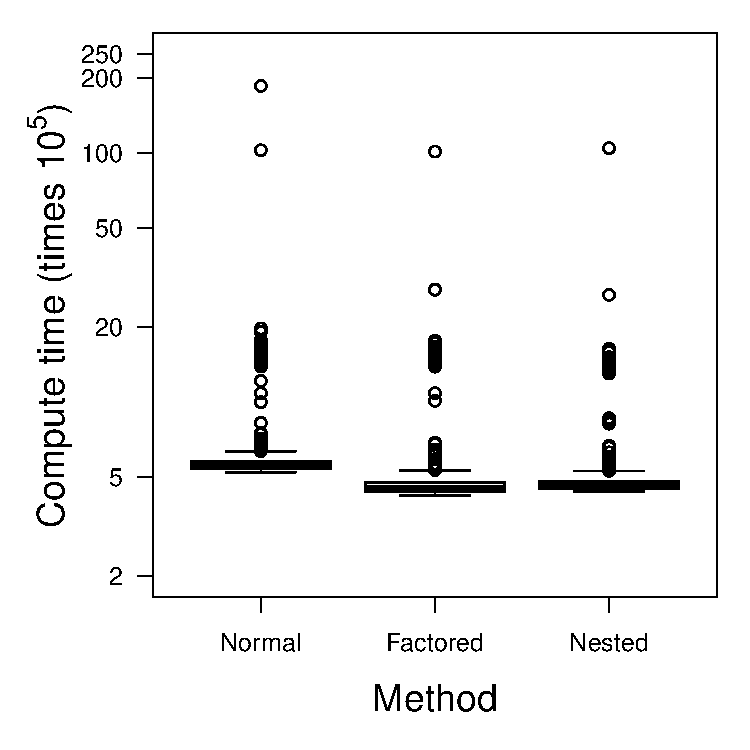
\includegraphics[width=0.65\textwidth]{polynomial_evaluation_plot.pdf}
\caption{Median computing times (measured execution time in microseconts) are 607.1064 for~\(f_1\),  511.8887 for~\(f_2\), and 516.9337 for~\(f_3\).}\label{fig::plots}
\end{figure}


\noindent With respect to class, you might ask yourself why we have emphasized nesting, but not factoring, when it comes to working with polynomials.

%
%\begin{table}[h!]\centering
%\begin{tabular}{cc}
%\hline
%\(r\) & Sample shape or example\\
%\hline\hline
%\(0<r<1\) & square root function (\(r=0.5\))\\
%\(r=1\) & linear function \\
%\(r>1\) & quadratic or cubic functions
%\end{tabular}
%\end{table}

\end{document}